\documentclass{article}

% if you need to pass options to natbib, use, e.g.:
% \PassOptionsToPackage{numbers, compress}{natbib}
% before loading rl_project.

% to compile a camera-ready version, add the [final] option, e.g.:
 \usepackage[final]{rl_project}

% to avoid loading the natbib package, add option nonatbib:
% \usepackage[nonatbib]{rl_project}

\usepackage[utf8]{inputenc} % allow utf-8 input
\usepackage[T1]{fontenc}    % use 8-bit T1 fonts
\usepackage{hyperref}       % hyperlinks
\usepackage{url}            % simple URL typesetting
\usepackage{booktabs}       % professional-quality tables
\usepackage{amsfonts}       % blackboard math symbols
\usepackage{nicefrac}       % compact symbols for 1/2, etc.
\usepackage{microtype}      % microtypography
\usepackage{graphicx}


% Give your project report an appropriate title!

\title{RL Lunar Lander}


% The \author macro works with any number of authors. There are two
% commands used to separate the names and addresses of multiple
% authors: \And and \AND.
%
% Using \And between authors leaves it to LaTeX to determine where to
% break the lines. Using \AND forces a line break at that point. So,
% if LaTeX puts 3 of 4 authors names on the first line, and the last
% on the second line, try using \AND instead of \And before the third
% author name.

\author{
  Andrej Lukic
  \\
  Department of Computer Science\\
  University of Bath\\
  Bath, BA2 7AY \\
  \texttt{al2274@bath.ac.uk} \\
  %% examples of more authors
  %% \And
  %% Coauthor \\
  %% Affiliation \\
  %% Address \\
  %% \texttt{email} \\
  %% \AND
  %% Coauthor \\
  %% Affiliation \\
  %% Address \\
  %% \texttt{email} \\
  %% \And
  %% Coauthor \\
  %% Affiliation \\
  %% Address \\
  %% \texttt{email} \\
  %% \And
  %% Coauthor \\
  %% Affiliation \\
  %% Address \\
  %% \texttt{email} \\
}

\begin{document}

\maketitle

\section{Problem Definition}
The problem chosen for this assignment is the Lunar Lander problem because landing a small rocket on the moon is a bit correlated with my interest in flight controllers used in custom made drones. The environment for testing the algorithm is freely available on the \href{https://gymnasium.farama.org}{Gymnasium} web site (it's an actively maintained fork of the original \href{https://github.com/openai/gym}{OpenAI Gym} developed by Oleg Klimov.

The \href{https://gymnasium.farama.org/environments/box2d/lunar_lander/}{Lunar Lander}  is a classic rocket trajectory optimisation problem (\href{https://gymnasium.farama.org/environments/box2d/lunar_lander/}{comprehensive environment description is found on the gymnasium web site} ). In the simulation, the spacecraft has a main engine and two lateral boosters that can be used to control its descent and the orientation of the spacecraft. The spacecraft is subject to the moon's gravitational pull, and the engines have an unlimited amount of fuel. The spacecraft must navigate to the landing spot between two flags at coordinates (0,0) without crashing. Landing outside of the landing pad is possible. The lander starts at the top center of the viewport with a random initial force applied to its center of mass. The environment has 4 discrete actions: 

\begin{itemize}
  \item 0: do nothing
  \item 1: fire left orientation engine
  \item 2: fire main engine
  \item 3: fire right orientation engine
\end{itemize}

The state is an 8-dimensional vector: the coordinates of the lander in x \& y, its linear velocities in x \& y, its angle, its angular velocity, and two booleans that represent whether each leg is in contact with the ground or not.

After every step a reward is granted. The total reward of an episode is the sum of the rewards for all the steps within that episode.

For each step, the reward:
\begin{itemize}
  \item is increased/decreased the closer/further the lander is to the landing pad.
  \item is increased/decreased the slower/faster the lander is moving.
  \item is decreased the more the lander is tilted (angle not horizontal).
  \item is increased by 10 points for each leg that is in contact with the ground.
  \item is decreased by 0.03 points each frame a side engine is firing.
  \item is decreased by 0.3 points each frame the main engine is firing.
\end{itemize}

The episode receive an additional reward of -100 or +100 points for crashing or landing safely respectively. An episode is considered a solution if it scores at least 200 points.

The episode finishes if:
\begin{itemize}
  \item the lander crashes (the lander body gets in contact with the moon);
  \item the lander gets outside of the viewport (x coordinate is greater than 1);
  \item the lander is not awake. From the Box2D docs, a body which is not awake is a body which doesn’t move and doesn’t collide with any other body:
\end{itemize}

\section{Background}
The lunar lander environment features a relatively big, continuous state space. This already narrows down the selection of the appropriate algorithms to those families of algorithms that don't assume the perfect knowledge of the environment, e.g. dynamic programming would most likely not be feasible since it would not be possible to efficiently estimate the state-value function. Monte-Carlo methods on the other hand don't require the perfect knowledge of the environment and learn from the agent's experiences. They would therefore be a more suitable candidate for a large state space. However a drawback of Monte Carlo methods is that they require a full completed episode to learn and so the convergence might be too slow to efficiently solve the problem. Additionally they need to store the action-value function and the complete list of returns for every episode in memory and would potentially require lots of space. Another family of methods are the Temporal-difference methods which solve the first drawback of the Monte-Carlo methods and can learn at every step since they make use of bootstrapping while still relying on agent's experiences like the Monte-Carlo methods. Therefore the agent can improve even before reaching the goal state which is an important aspect for environments like Lunar Lander where an agent might take many steps before reaching a goal. Q-learning is one such algorithm, that is also is an off-policy method so it isn't limited to learning the policy it's following while learning the optimal policy. The speed of convergence of the Q-learning can be further improved up by remembering past state transitions and simulating moves and thus speeding up the learning process as in the Dyna-Q algorithm. All of the mentioned methods however have one thing in common. They assume a finite state and action space and therefore can rely on tabular representation of the Q-value estimate. In order to scale pas vt the finite number of states even to improve the performance of agents in environments with a large number of states a function approximation for the state-value function can be used instead. One such method was used by the DeepMind that learned to play Atari games by using a neural network as a function approximator. This way the size of the state space does not matter any more a problem since we have no Q table that needs to be maintained in the memory. The agent still learns from experiences as in the MC and TD methods and is not limited to completing an episode. In this project two such algorithms were tested on the Lunar Lander problem, DQN with one and DQN with two neural networks.
 
\section{Method}
To solve the Lunar Lander problem two very similar deep RL methods were used. Deep Q-learning (DQN) is essentially a Q-learning algorithm with an approximation of the Q-value function that receives a state as an input and returns actions with their q-values instead of the old tabular Q-value function that simply maps a state-action pair to a Q value. A neural network is used here as a function approximator. In the case of a DQN a single neural network is used for two important steps, choosing agent's actions as well as for evaluating the target Q values. This can lead to a so-called maximisation bias which means that a maximum over estimated values is used implicitly as an estimate of the maximum value. A further example of such a bias is provided in Sutton and Barto (2018, p.134) which illustrates situations in which a wrong action would be chosen by an agent due to this effect. To overcome this challenge an improved version of a DQN is such that a separate neural network is added for updating the target values. This second neural network has the same shape and architecture as the one used for the action-selection and is periodically updated with the weights of the action-selection network. Such reduced frequency of updates to the target network means that the target values it is aiming at stay more stationary. Therefore the improvements to the action-selection network should be more efficient and we should see the agent converge faster and learn more robustly.

\section{Results}
Both algorithms (DQN and DDQN) converged nicely somewhere after the 369th episode (ie the average of the last 100 episodes exceeded 200 points). The final result of the agent landing the rocket can be seen by playing the following videos:

\begin{itemize}
  \item \href{https://youtu.be/csrk1gOcRPU}{Link to the video of an agent trained using DDQN (Experiment - M5) landing the rocket on the moon } 
  \item \href{https://youtu.be/Jb_1M_E6ofE}{Link to the untrained agent landing the rocket on the moon } 
\end{itemize}

The best performing approach out of those tested was a DDQN with a neural network with two hidden layers of size 256 neurons, batch size of 128 and the replay memory of 200000 transitions. It converged the fastest in the 369th episode \ref{fig:1}. The basic DQN also compared fairly well with the DDQN and the version with two 64 neuron layers converged at episode 461 \ref{fig:2}. On all the graphs red colour indicates the point on the graph where the average of the past 200 episodes exceeded 200 points and the line is marked with red colour from that point onwards.

\begin{figure}[!h]
  \centering
	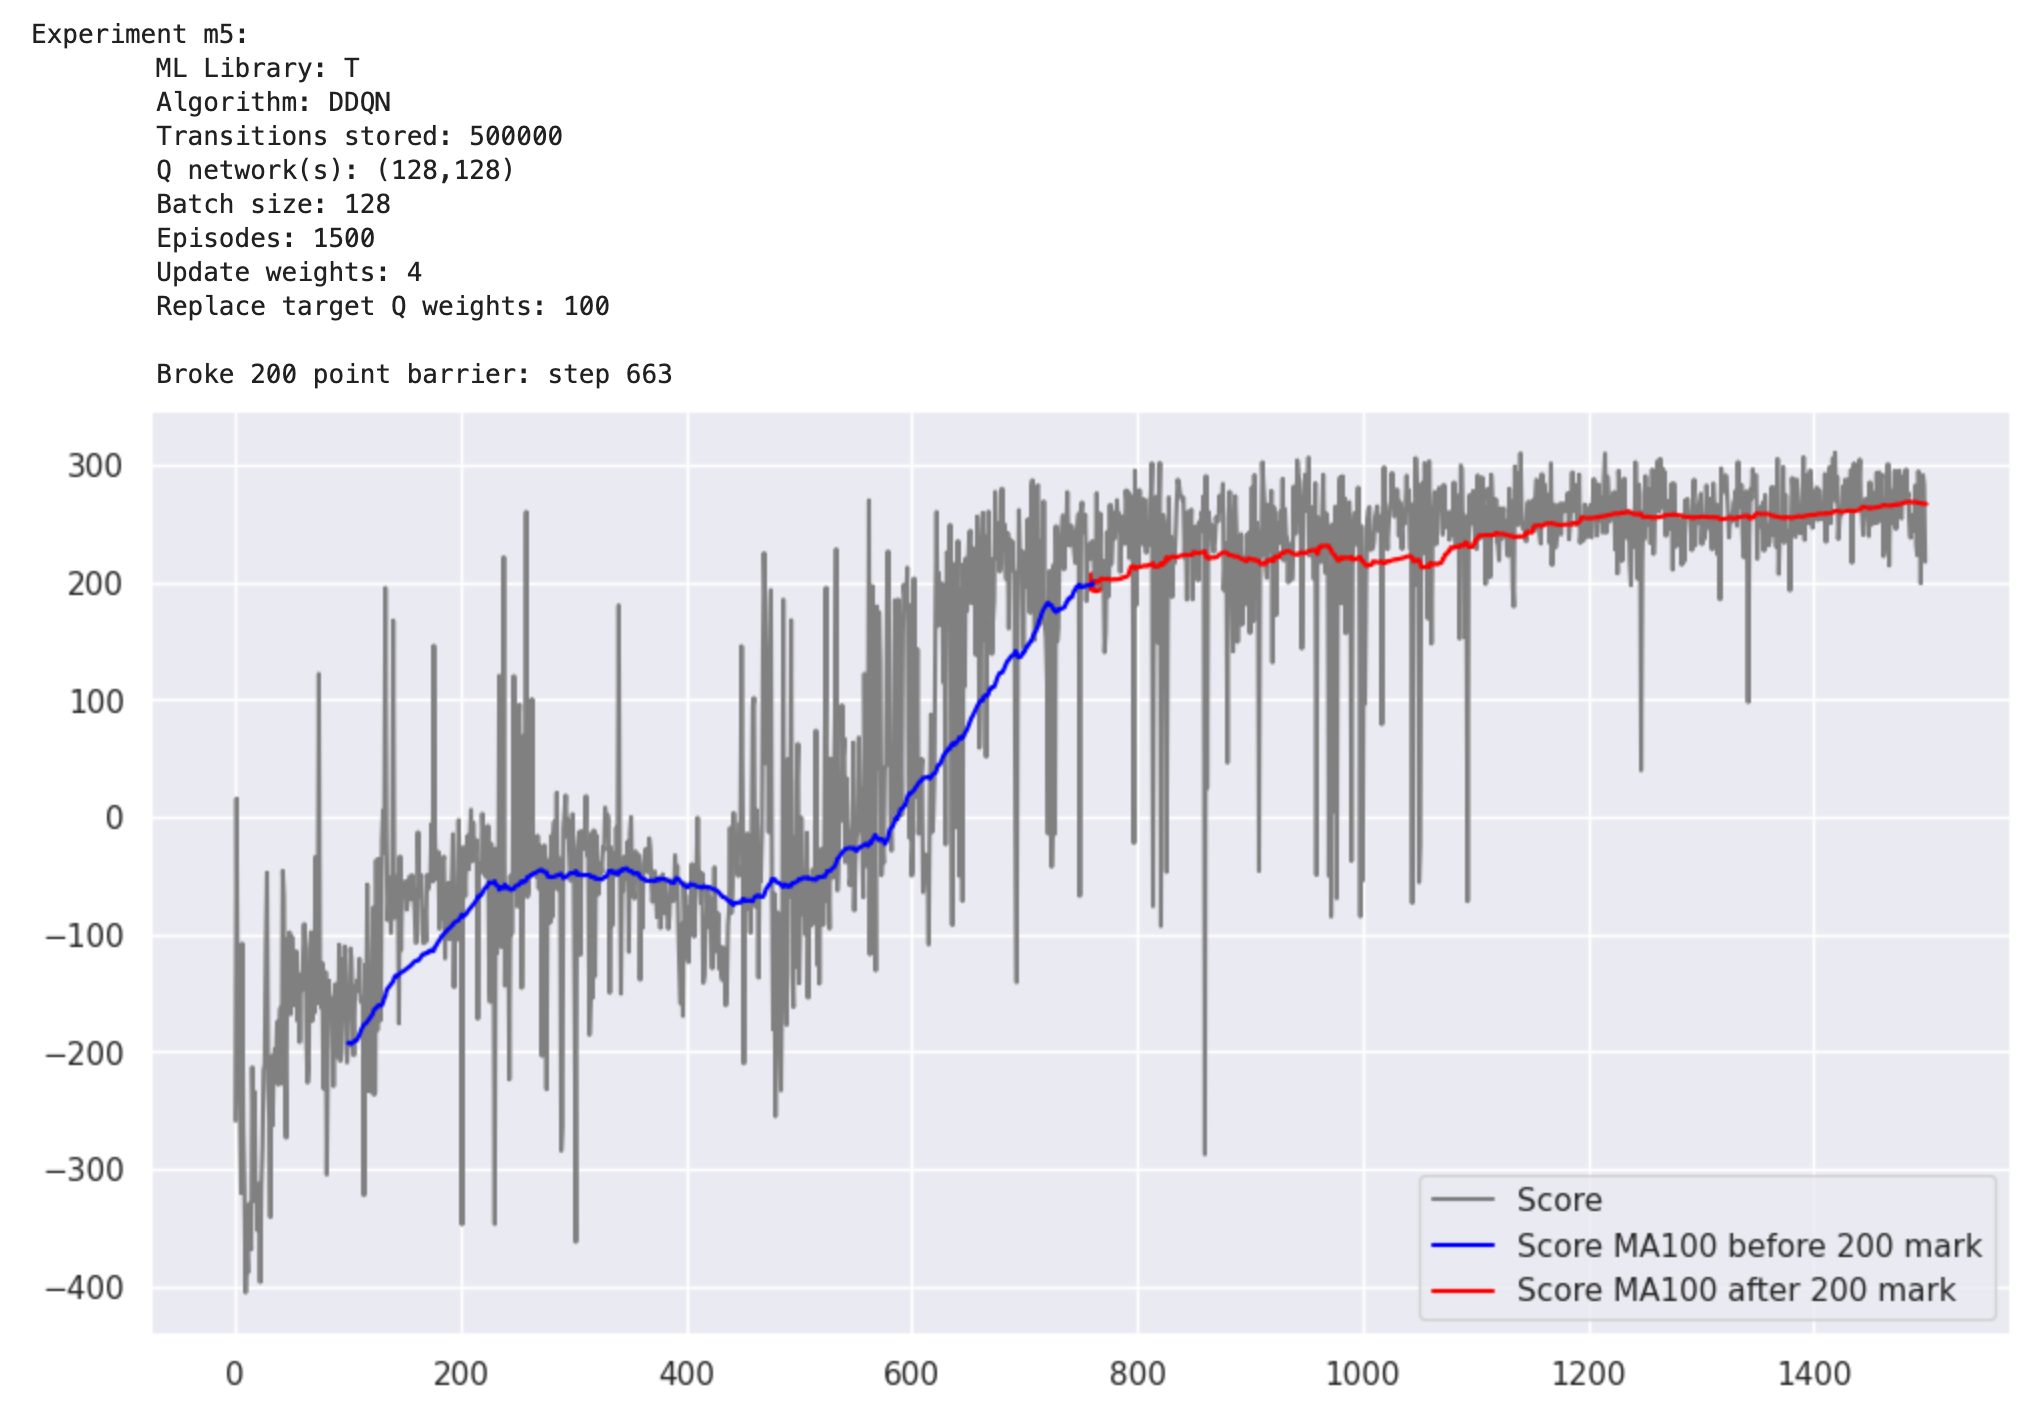
\includegraphics[width=1.0\textwidth]{figures/m5.png}
  \caption{DDQN, 200000 experiences, NN(256,256), batch size 128, 1500 episodes, learn every 4th step N/A}
  \label{fig:1}
\end{figure}

\begin{figure}[!h]
  \centering
	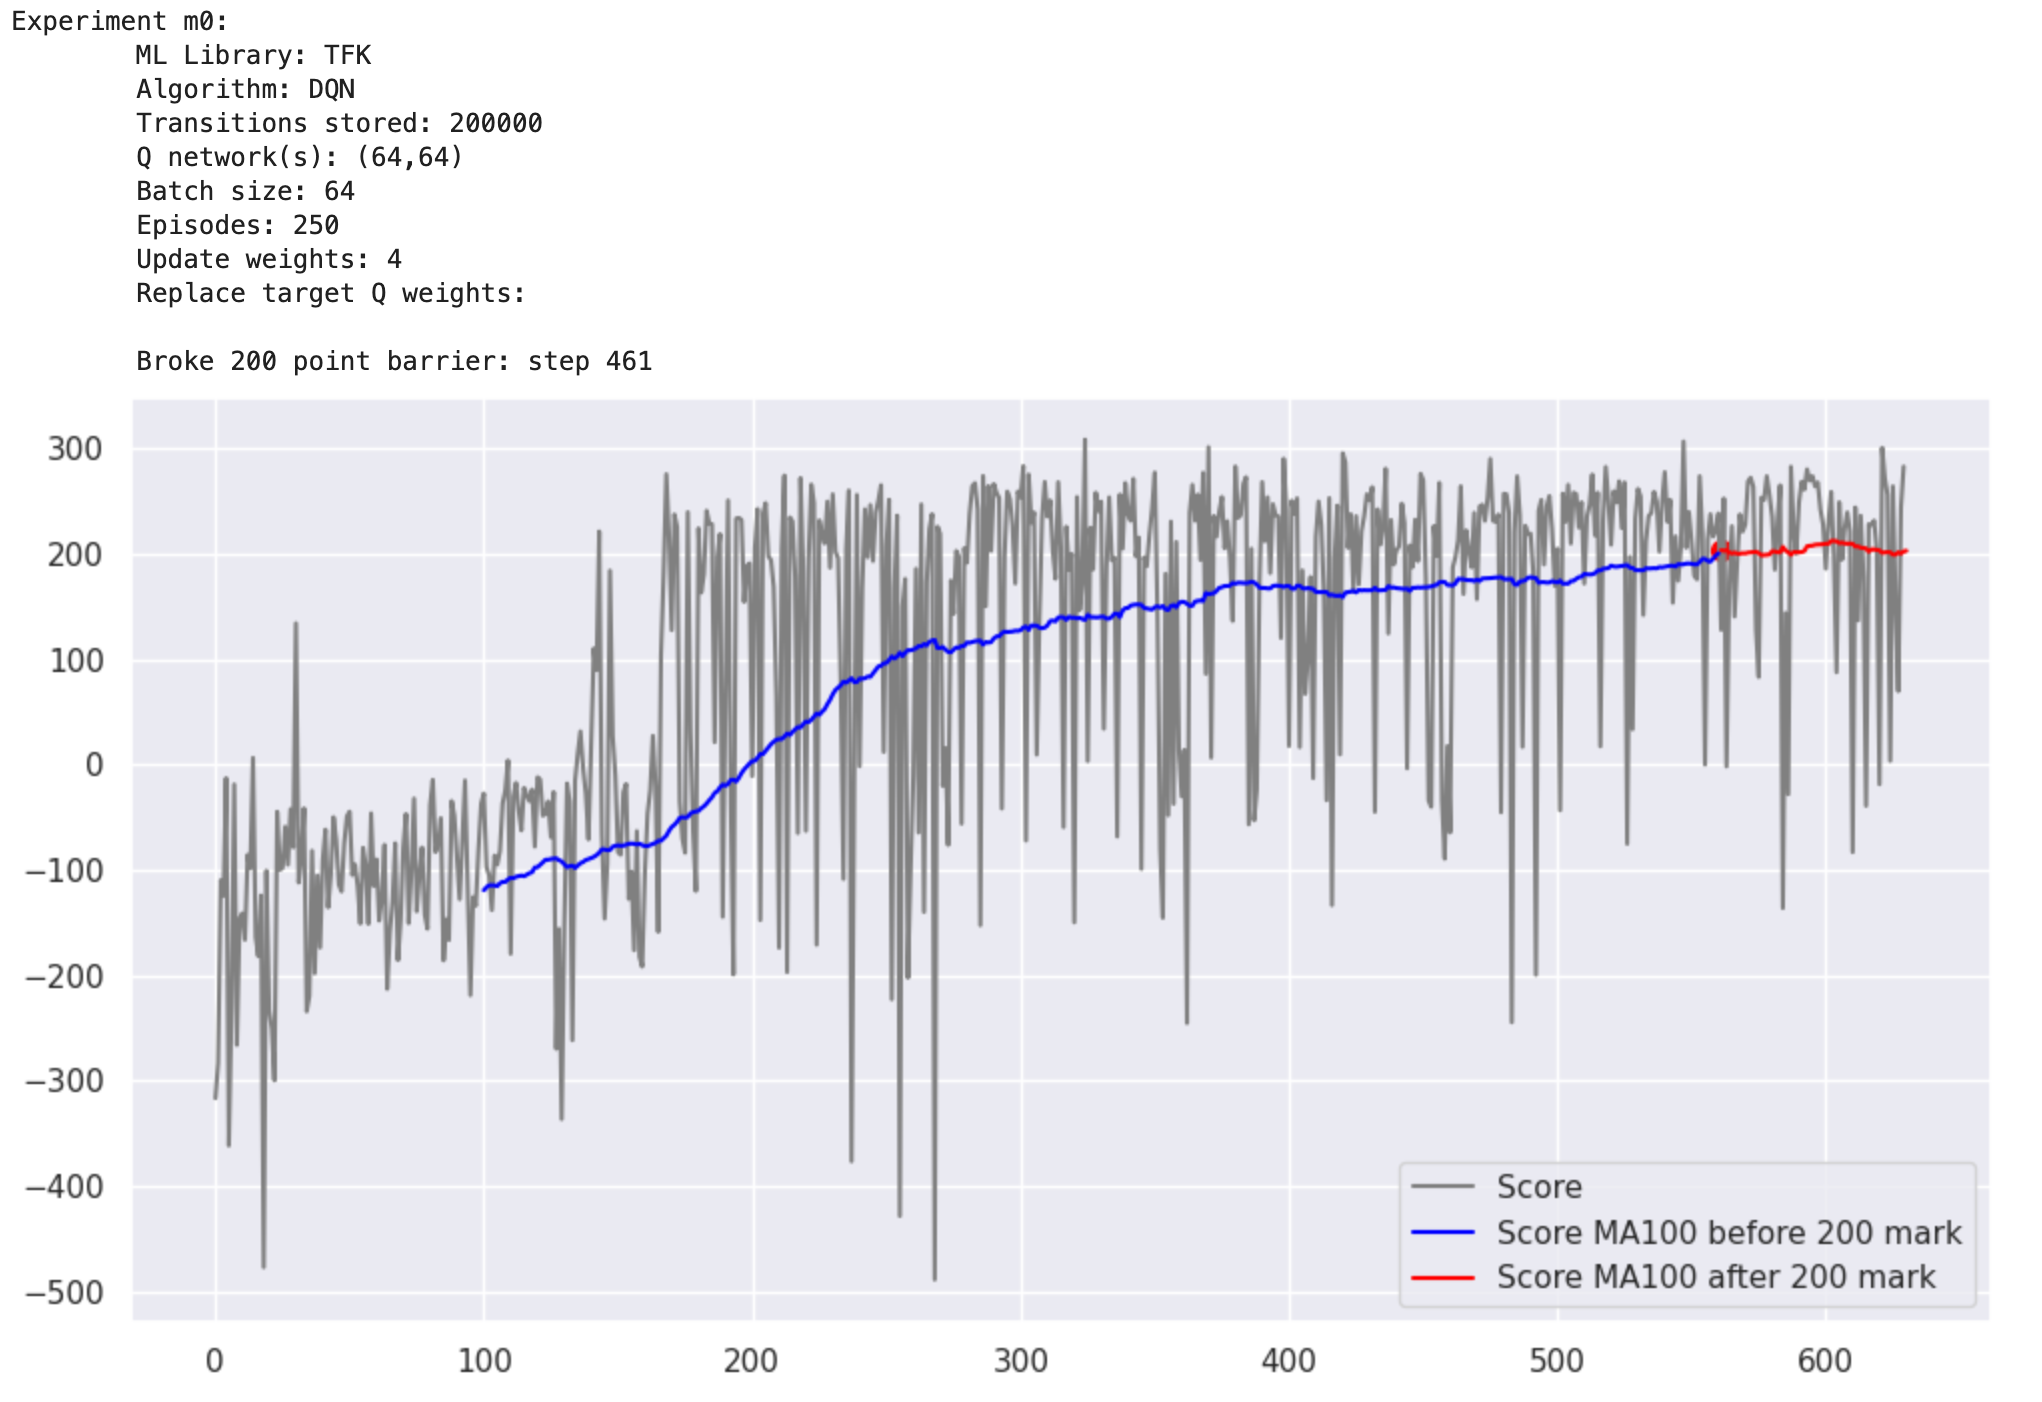
\includegraphics[width=1.0\textwidth]{figures/m0.png}
  \caption{DQN, 200000 experiences, NN(64,64), batch size 64, 629 episodes, learn every 4th step N/A}
  \label{fig:2}
\end{figure}

The experiments showed that the network hidden layer width had a big impact on the speed of converging but the depth not so much. In the figure \ref{fig:3} a rolling average with the window 100 can be seen and it shows that the neural network with only two hidden layers and 64 neurons per layer performs the worst. Increasing depth and also width drastically improves performance however also increases the computational complexity and it seems that the width of 256 neurons gives the best performance.

\begin{figure}[!h]
  \centering
	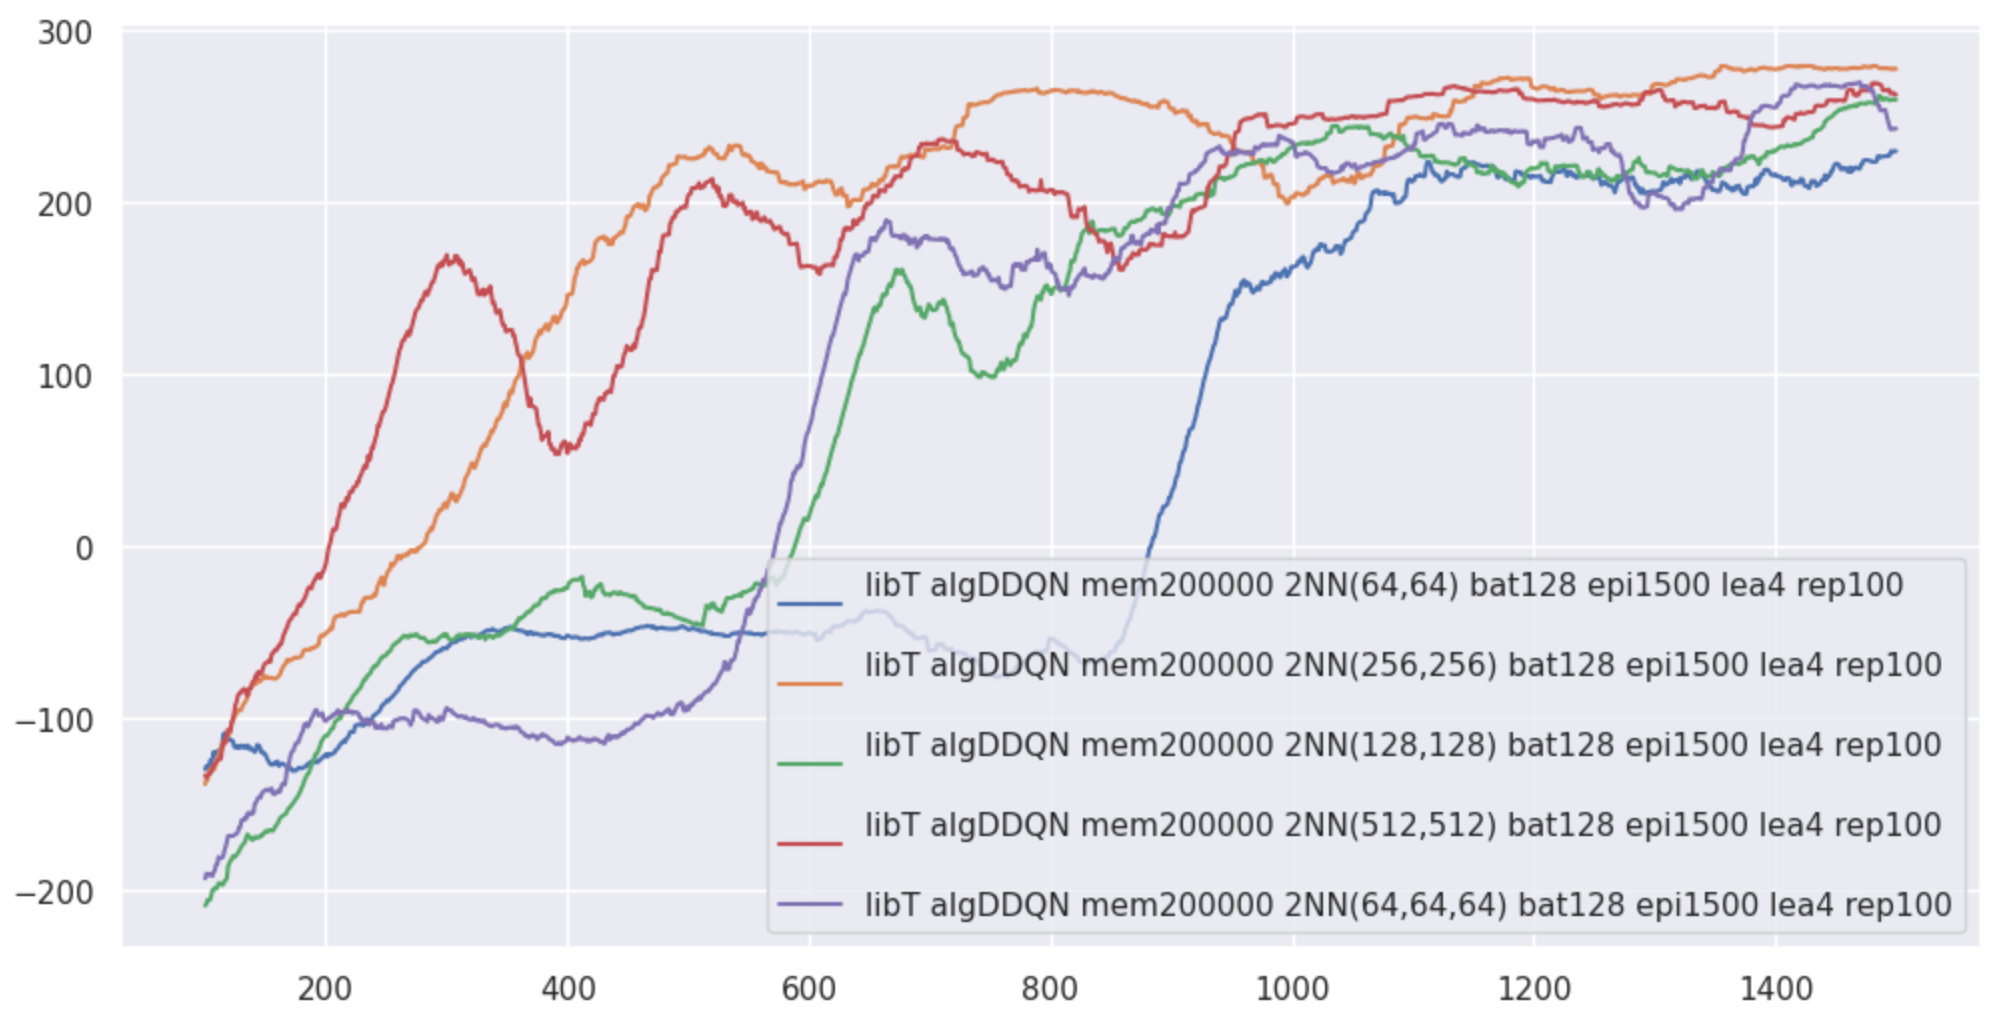
\includegraphics[width=1.0\textwidth]{figures/nnwidth.png}
  \caption{NN with too little neurons seem to converge too late}
  \label{fig:3}
\end{figure}

\section{Discussion}
After the technical issues were resolved (more on this in the last section) the problem was easily solved using the DDQN / DQN methods. Using the trained agent to repeatedly land the rocket shows impressive results and even when the landing is not perfect the rocket usually does not end up crashing. 

\section{Future Work}
Since the Lunar Lander is not such a complex problem it would be interesting to compare the deep RL methods to the simpler methods from the family of the temporal difference algorithms and see how much faster / slower the deep learning approach converges compared to SARSA or the Dyna-Q. What also be interesting is do a more extensive hyper parameter tuning and determine what the best neural network architecture is e.g. would a convolutional network or a duelling network perform better.

\section{Personal Experience}
The implementation was first written for TensorFlow and Keras which performed poorly. The combination of TensorFlow / Keras and the gymnasium library have no working combination on a M1 Macbook so the training was performed on a remote computer in Jupyter Labs. However the training process ran  slow and consumed more memory with every episode until it ran out of available memory. The only way the models could be trained was to periodically dump the neural network weights as well as the internal buffer state to disk and reload them after the process crashed. In this way the training process picked up where it left off and continued improving the model. The DQN agent in \ref{fig:2} was trained in 10 separate sessions over two days to reach roughly the episode 700, each session ending in out of memory exception.  After extensive debugging and benchmarking every part of the agent including rewriting the replay buffer several times between a pure numpy implementation and the dequeue buffer there was one culprit left. There seems to be some undetermined issue with the TensorFlow/Keras running on my hardware or a programming mistake on my side. The TensorFlow/Keras neural network implementation was replaced by Pytorch and the performance increased 100 fold. All the experiments excluding the first one were subsequently run using the Pytorch approach and are able to reach the episode 1500 under one hour. Both implementations are included in the project.

\section*{References}
\small Sutton, R.S., Bach, F., and Barto, A.G., 2018. Reinforcement learning: An introduction. Massachusetts: MIT Press Ltd. 

\normalsize
\newpage

\end{document}
